\documentclass[11pt]{article}
\usepackage[T1]{fontenc}
\usepackage{mathpazo}
\usepackage[margin=1.05in]{geometry}
\usepackage{amsmath,amssymb,amsthm,mathtools}
\usepackage{microtype}
\usepackage{enumitem}
\usepackage{needspace}
\usepackage{xcolor}
\usepackage{tikz}
\usetikzlibrary{arrows.meta,positioning,decorations.pathreplacing}
\usepackage[colorlinks=true,linkcolor=blue!55!black,citecolor=blue!55!black,urlcolor=blue!55!black]{hyperref}
\hypersetup{pdftitle={A closed Ricci flow with bounded scalar curvature and finite-time curvature blowup},pdfauthor={OpenAI}}
\newtheorem{theorem}{Theorem}[section]
\newtheorem{proposition}[theorem]{Proposition}
\newtheorem{lemma}[theorem]{Lemma}
\newtheorem{corollary}[theorem]{Corollary}
\theoremstyle{definition}
\newtheorem{definition}[theorem]{Definition}
\theoremstyle{remark}
\newtheorem{remark}[theorem]{Remark}
\numberwithin{equation}{section}
\DeclareMathOperator{\Ric}{Ric}
\DeclareMathOperator{\Rm}{Rm}
\DeclareMathOperator{\tr}{tr}
\DeclareMathOperator{\diag}{diag}
\newcommand{\D}{\mathcal D}
\newcommand{\Sp}{\mathbb S}
\newcommand{\Ut}{\widetilde U}
\newcommand{\Zt}{\widetilde Z}
\newcommand{\dt}{\partial_t}
\newcommand{\const}{C}
\setlist{itemsep=3pt,topsep=5pt}
\setlength{\emergencystretch}{2em}
\title{A closed Ricci flow with bounded scalar curvature\\and finite-time curvature blowup}
\author{OpenAI}
\date{September 24, 2026}
\begin{document}
\maketitle
\begin{abstract}
We disprove the scalar-curvature extension conjecture in its unrestricted
all-dimensions form. In sufficiently high dimension, we construct a Ricci
flow on a closed manifold whose scalar curvature remains uniformly bounded
while full curvature diverges at a finite maximal time. In one fixed
sufficiently high dimension, the examples have two-sided power-law curvature
blowup with arbitrarily large exponents.
\end{abstract}

\section{Introduction}

A Ricci flow on a smooth manifold is a family of Riemannian metrics
\(g(t)\) satisfying \(\partial_tg=-2\Ric_g\). Here a closed manifold
is compact and has no boundary, \(\Rm\) denotes its full curvature
tensor, and \(R=\operatorname{tr}_g\Ric\) denotes scalar curvature.
A smooth Ricci flow on a closed manifold can fail to extend at a finite time
only if its full curvature becomes unbounded~\cite{Hamilton1995}.
The scalar-curvature extension conjecture asks whether scalar curvature
alone must detect such a singularity; see~\cite[p.~756]{Bamler2018}.
A uniform bound for the Ricci tensor is sufficient for extension
by \v{S}e\v{s}um's Theorem~\cite{Sesum2005}, but the trace of that tensor
contains substantially less information. The question concerns smooth
extension on the original manifold; continuation through a singular space
is a different conclusion.

Bounded scalar curvature imposes a necessary restriction on the rate of
full-curvature blowup. Wang proved that, at a finite singular time \(T\),
the product of \(T-t\), the square root of the maximum full curvature,
and the square root of the maximum absolute scalar curvature has a
strictly positive upper limit~\cite[Theorem~3]{Wang2012}.
Consequently, a closed flow with bounded scalar curvature must satisfy
\[
\limsup_{t\uparrow T}(T-t)^2\max_M|\Rm|(\cdot,t)>0.
\]
This is a subsequential restriction; it does not assert a lower bound at
every sufficiently late time. It explains why examples with curvature
concentration faster than the parabolic rate are relevant to the
extension question.

Symmetry has made it possible to construct and study singularities with
several distinct geometric scales. Angenent and Knopf constructed
rotationally symmetric neckpinches on spheres~\cite{AK2004}.
A finite-time singularity is of
\emph{Type II} when \((T-t)\max_M|\Rm|\) is unbounded.
Gu and Zhu constructed rotationally symmetric Type-II singularities on
spheres~\cite{GuZhu2008}. Angenent, Isenberg, and Knopf later constructed
degenerate neckpinches with prescribed rates, a Bryant-soliton tip model,
and a shrinking-cylinder parabolic model~\cite{AIK2015}.
The Type-II constructions establish that full curvature can concentrate faster
than the parabolic scale, but do not supply the scalar bound in
Theorem~\ref{thm:main}.

Stolarski constructed closed, doubly warped Ricci flows that develop
conical singularities with arbitrarily fast curvature blow-up and approach
a Ricci-flat cone at the parabolic scale~\cite{Stolarski2019}.
Stolarski's discussion identifies bounded scalar curvature as a possible
feature of these examples. The construction does not supply the
scalar-curvature bound proved below.
We use its quantitative profile estimates and establish that bound for a
choice of sufficiently large dimension and mode index.
The geometric cap models considered in his formal discussion belong to
the cohomogeneity-one Ricci-flat setting developed by
B\"ohm~\cite{Bohm1999,Stolarski2019}. Our cap estimate uses only
the quantitative construction inputs stated in
Proposition~\ref{prop:input}; it does not require convergence to a
prescribed complete cap metric.

\begin{theorem}\label{thm:main}
There are an integer \(q\ge10\), a time \(T>0\), and a smooth Ricci flow
\(g(t)\), \(0\le t<T\), on the closed connected manifold
\(M=\Sp^2\times\Sp^{q+1}\), with smooth initial metric, such that
\[
\sup_{M\times[0,T)}|R_{g(t)}|<\infty,
\qquad
\lim_{t\uparrow T}\max_M|\Rm_{g(t)}|=\infty.
\]
In particular, \(T\) is the finite maximal existence time of this flow.
\end{theorem}

Theorem~\ref{thm:main} refutes this conjecture in its unrestricted
all-dimensions formulation: the assertion that every finite-time
singularity of a closed Ricci flow in dimension at least four has unbounded
scalar curvature. The example is in sufficiently high dimension; no
dimension-four conclusion is asserted.

The estimates also determine the full-curvature rate of the examples.
Corollary~\ref{cor:rates} gives two-sided power-law bounds with an unbounded
discrete set of exponents, while the dimension remains fixed. Thus the
scalar bound is compatible with arbitrarily fast power-law Type-II
singularities, and the upper rate is controlled as well as the lower rate.

\subsection*{The two scales and the proof}

The examples have two sphere factors whose radii vary along an interval.
Off the two pole orbits the metric is
\[
ds^2+\phi(s,t)^2g_{\Sp^2}+r(s,t)^2g_{\Sp^q},
\]
where \(s\) is arclength at the indicated time and the sphere metrics
have sectional curvature one. At each endpoint the \(\Sp^q\) factor
collapses smoothly, leaving a positive-radius \(\Sp^2\) orbit.
The singularity develops when that remaining orbit also shrinks.

Write \(\delta=T-t\). The parabolic length scale is \(\sqrt\delta\),
where the rescaled metric closely approximates a Ricci-flat cone.
The smaller cap scale is \(\theta=\delta^\sigma\), with a fixed
exponent \(\sigma>1/2\) supplied by the construction. These two
scales have different roles: the cone approximation gives small Ricci
curvature on fixed parabolic annuli, whereas smoothness at the pole must
be controlled on the cap scale. A small Ricci tensor at the larger scale
does not by itself control the smaller cap.

The additional estimates have two features. First, Stolarski's strict
one-sided comparison with the cone and monotonicity of a logarithmic
slope, together with the ordinary scalar lower bound, control the size of
the cap. We adapt the scalar-sign obstruction in his
Proposition~5.3~\cite{Stolarski2019} to obtain this quantitative estimate.
Curvature
point-picking then gives a full-curvature bound without assuming convergence
to a cap model. Second, on radial cylinders moving with the dominant drift,
one-dimensional parabolic estimates give a Ricci reaction bound with leading
coefficient \(2q\). The corresponding diffusion coefficient leaves a positive
margin in large dimension. This yields
\( |\Ric|\le Cr^{-e}\) for an exponent \(0<e<1\), where \(r\) is
the radius of the \(\Sp^q\) factor in the doubly warped metric.
The square of this bound admits a bounded scalar-curvature supersolution.
These are the new estimates beyond the imported singular-flow construction.

Section~\ref{sec:construction} states the precise construction input and
translates its scales. Section~\ref{sec:geometry} obtains the warping
identities, the strict cone gap, and the parabolic-annulus estimates.
Section~\ref{sec:cap} proves the cap and radius curvature bounds by two
curvature-record arguments and Shi's derivative estimates.
Section~\ref{sec:reaction} proves the dimension-explicit reaction bound;
the analytic estimates take place in one space dimension, which is what
keeps their constants independent of \(q\).
Section~\ref{sec:barriers} fixes the parameters in order and completes
the Ricci and scalar comparisons, then records the resulting curvature rates.

\paragraph{Conventions.}
All tensor norms and geometric differential operators are taken with respect
to \(g(t)\), and \(\dt g=-2\Ric\).
The unit sphere has sectional curvature one. A constant \(C\) may change
between occurrences. Unless explicitly stated otherwise, it may depend on
all fixed parameters of the chosen flow, but never on \(t\uparrow T\).
Constants used to choose the dimension will be identified as independent
of both the dimension parameter \(q\) and the mode index \(k\).

\section{The construction used as input}\label{sec:construction}

We record precisely the part of Stolarski's construction that is needed.
The role of this input is to produce a single smooth singular flow with
compatible inner signs and cone profiles. The curvature estimates proved
in the later sections will be consequences of these data.
Throughout, set \(p=2\) and write
\begin{equation}\label{eq:parameters}
\begin{gathered}
m=p+q,\qquad A^2=\frac{p-1}{m-1},\qquad B^2=\frac{q-1}{m-1},\\
d=\frac{m-1-\sqrt{(m-1)(m-9)}}2,\qquad
\nu=k-d/2,\qquad \sigma=k/d.
\end{gathered}
\end{equation}
Here \(q\ge10\), and \(k\) is a sufficiently large even positive integer.
In particular \(\nu>0\). We take \(A,B>0\) and use the time-dependent scales
\begin{equation}\label{eq:scales}
\delta=T-t,\qquad \tau=-\log\delta,\qquad
\theta=\delta^\sigma,\qquad \gamma=r/\sqrt\delta.
\end{equation}
The dimension of the manifold is \(m+1\).
The identities \(\nu/d=\sigma-1/2\) and
\(\sqrt\delta\,\delta^{\nu/d}=\theta\) relate the two scales.

\begin{proposition}[Construction input]\label{prop:input}
For the parameters above, Stolarski's construction supplies a smooth Ricci
flow up to a finite time \(T\) on \(\Sp^p\times\Sp^{q+1}\) with the
following properties, after translating its starting time to zero.

\begin{enumerate}[label=\textup{(\roman*)}]
\item Off the two pole orbits it has the form
\[
g=ds^2+\phi^2g_{\Sp^p}+r^2g_{\Sp^q}.
\]
Here \(s\) is radial arclength at each time. The metric is invariant under
reflection exchanging the poles. On each open hemisphere, oriented from
its pole toward the equator, \(r_s>0\). At a pole, \(r=0\), \(r_s=1\),
and \(\phi_s=0\); the usual odd and even polar expansions hold for \(r\)
and \(\phi\), respectively, and \(\phi>0\) for every \(t<T\).

\item Write \(u=\log\phi\), \(z=r_s^2\), and
\[
\Ut=\log\frac{\phi}{(A/B)r},\qquad \Zt=z-B^2.
\]
There are positive tolerances \(\eta_j^U,\eta_j^Z\), large fixed numbers
\(1<Y_1\le Y_2\), and constants \(M_0>0\), \(0<\beta<1/2\), such that
for \(j=0,1,2\),
\begin{equation}\label{eq:profile-bounds}
\begin{aligned}
\left|\partial_\gamma^j(\Ut-\delta^\nu U_k)\right|
&\le\eta_j^U\delta^\nu
       \bigl(\gamma^{-d-j}+\gamma^{2k-d}\bigr),\\
\left|\partial_\gamma^j(\Zt-\delta^\nu Z_k)\right|
&\le\eta_j^Z\delta^\nu
       \bigl(\gamma^{-d-j}+\gamma^{2k-d}\bigr).
\end{aligned}
\end{equation}
The first estimate holds from \(Y_1\delta^{\nu/d}\) to
\(M_0e^{\beta\tau}\), and the second from \(Y_2\delta^{\nu/d}\) to that
upper endpoint, within the hemisphere. The profiles are smooth on
\(\gamma>0\). The function \(U_k\) is \(\gamma^{-d}\) times a polynomial
of degree \(k\) in \(\gamma^2\), with positive leading coefficients at
zero and infinity:
\[
U_k(\gamma)\sim c_1\gamma^{-d}\quad(\gamma\downarrow0),\qquad
U_k(\gamma)\sim c_2\gamma^{2k-d}\quad(\gamma\to\infty),\qquad c_1,c_2>0.
\]
Also \(Z_k(\gamma)=O_{q,k}(\gamma^{-d})\) as \(\gamma\downarrow0\).

\item For all sufficiently late times, putting \(f=ru_r\), one has
\begin{equation}\label{eq:inner-inputs}
\begin{gathered}
\phi/r\ge A/B,\qquad 0\le f\le1,\qquad f_r\ge0
       \quad(0<r\le Y_1\theta),\\
B^2\le z\le1\quad(0<r\le Y_2\theta).
\end{gathered}
\end{equation}
These inner intervals lie strictly below the equator.

\item At the initial time \(\tau_0=-\log T\), the same weighted profile
bounds hold up to an initial outer cutoff
\(G_{\mathrm{init}}=M_0e^{\beta_{\mathrm{init}}\tau_0}\),
where \(0<\beta_{\mathrm{init}}<1/2\), and \(\Ut\ge0\) beyond that
cutoff. The exponents are chosen in the ranges permitted by the
construction; in particular, one may take
\[
0<\beta<\frac{\nu}{2\nu+1}\le\beta_{\mathrm{init}}<\frac12.
\]
They are therefore distinct choices, not two arbitrary exponents.
The tolerances can be
chosen sufficiently small depending on \(q,k\). The inner cutoffs can then
be increased in order, first \(Y_1\) and then \(Y_2\); the initial
rescaled time can subsequently be increased. Each such increase is
subject only to lower-size requirements from the construction.
\end{enumerate}
\end{proposition}

\begin{proof}[Source and change of notation]
The existence statement is the solution furnished by Lemma~3.12 and the
proof of Theorem~1.1 in~\cite{Stolarski2019}. The weighted estimates are
Definition~3.1. The initial family is Definition~3.5 and Lemma~3.6,
with the outer conditions of Definition~3.2.
The inner inequalities are the Inner Region Barriers I in Definition~3.3,
as propagated by Lemmas~4.5--4.9 and explicitly invoked in the proof of
Theorem~4.3 on page~25. In particular that proof gives the barrier
conditions on the inner intervals; the shorter list in Definition~4.1
of its final class \(\mathcal P\) is not the only information being used.
The eigenprofile properties are Propositions~A.12, A.13, and A.21;
the parameter order is listed in Appendix~B.

For completeness, the initial weighted bounds hold up to the initial
expansion's own upper endpoint, not just the smaller propagated endpoint.
The lower \(U\)-modes in Definition~3.5 are \(\gamma^{-d}\) times
polynomials in \(\gamma^2\) of degree below \(k\).
By Propositions~A.10 and~A.19, the homogeneous lower \(Z\)-modes are
\(\gamma^2\) times polynomials, with growth exponents strictly below
\(2k-d\). Each of these finitely many modes and its first two
derivatives is therefore bounded by the corresponding weight in
\eqref{eq:profile-bounds} on all \(\gamma>0\).
Taking the lower-mode coefficient bound at the initial time to be
\(\epsilon_0\delta^\nu\), with \(\epsilon_0\) sufficiently small,
gives the required tolerances. This choice is compatible with the degree
argument in Lemma~3.10: the projection errors in Lemmas~6.13--6.14 can
subsequently be reduced by increasing the initial rescaled time.
Definition~3.5 imposes the outer conditions starting at that same initial
expansion endpoint. Thus the initial profile bounds and outer sign meet
at \(G_{\mathrm{init}}\); no identification of
\(\beta_{\mathrm{init}}\) with \(\beta\) is required.
The relation between their permitted ranges is specified in the proof
of Theorem~4.3, page~26, of~\cite{Stolarski2019}.

In the source's notation,
\(B^2\lambda_k=-\nu\), \(\alpha_k=\nu/d\), and
\(Y_1=\Upsilon_U\), \(Y_2=\Upsilon_Z\).
Thus \(\sqrt\delta\,Y_i e^{-\alpha_k\tau}=Y_i\theta\).
Moreover
\[
f=1+\gamma\Ut_\gamma,\qquad
f_r=\frac{\gamma}{\sqrt\delta}
   \left(\Ut_{\gamma\gamma}+\frac{\Ut_\gamma}{\gamma}\right),
\]
which translates the source's log-radius convexity into the last slope
inequality in~\eqref{eq:inner-inputs}.
The mode index \(k\) here is the index in the construction, rather than
the arbitrary curvature blow-up exponent in the statement of its
Theorem~1.1.
\end{proof}

\begin{remark}\label{rem:input-scope}
Proposition~\ref{prop:input} is the external existence input to this paper.
We do not import a scalar-curvature upper bound, a full-curvature bound at
the cap scale, or convergence to a particular complete cap metric.
The estimates establishing those curvature bounds are given below.
\end{remark}

\section{Geometric identities and profile consequences}\label{sec:geometry}

We now extract three consequences needed in the curvature estimates:
uniform bounds for the warping slopes, a strict inner separation from the
cone, and small Ricci curvature on fixed parabolic annuli. We distinguish
time differentiation at a fixed point of the manifold from differentiation
at a fixed value of the evolving radius \(r\).

\subsection{Warping equations}

Let \(x\) be a radial coordinate fixed on the manifold, so that
\(ds=\chi(x,t)\,dx\). Subscripts \(s\) denote arclength differentiation
at the indicated time. On a regular orbit the sectional curvatures are
\begin{equation}\label{eq:sectional}
\begin{gathered}
h=-\phi_{ss}/\phi,\qquad h_q=-r_{ss}/r,\qquad
j=(1-\phi_s^2)/\phi^2,\\
\ell=(1-r_s^2)/r^2,\qquad
\mu=-\phi_s r_s/(\phi r).
\end{gathered}
\end{equation}
They correspond, respectively, to radial--\(\Sp^p\), radial--\(\Sp^q\),
\(\Sp^p\)-tangent, \(\Sp^q\)-tangent, and mixed planes. These formulas
also follow directly by computing the connection of the warped metric.
The Ricci eigenvalues in the radial and the two fiber directions are
\begin{equation}\label{eq:ricci-eigenvalues}
\lambda_0=ph+qh_q,\qquad
\lambda_p=h+(p-1)j+q\mu,\qquad
\lambda_q=h_q+(q-1)\ell+p\mu.
\end{equation}
Consequently
\begin{equation}\label{eq:warping-flow}
\begin{aligned}
\dt\big|_x r&=r_{ss}+(q-1)(r_s^2-1)/r+p\phi_s r_s/\phi,\\
\dt\big|_x\phi&=\phi_{ss}+(p-1)(\phi_s^2-1)/\phi+q r_s\phi_s/r,\\
[\dt\big|_x,\partial_s]&=\lambda_0\partial_s.
\end{aligned}
\end{equation}
These are also the usual doubly warped Ricci-flow equations
in~\cite[Section~2]{Stolarski2019}.

\begin{lemma}[Global elementary bounds]\label{lem:gradients}
For each flow in Proposition~\ref{prop:input}, there is a time-independent
constant \(C\) such that
\[
r\le C,\qquad |r_s|+|\phi_s|\le C.
\]
In particular, \(r\) is uniformly Lipschitz in the metric \(g(t)\).
Also \(R\ge-C\) throughout the flow.
\end{lemma}

\begin{proof}
At a positive maximum of \(r\), its first derivative vanishes and
\eqref{eq:warping-flow} gives \(r_t\le-(q-1)/r\).
Differentiating the first equation with the stated commutator gives
\begin{equation}\label{eq:slope-flow}
\begin{split}
\dt\big|_x r_s={}&(r_s)_{ss}
 +\left(p\frac{\phi_s}{\phi}+(q-2)\frac{r_s}{r}\right)(r_s)_s\\
&+\left[\frac{(q-1)(1-r_s^2)}{r^2}
       -p\frac{\phi_s^2}{\phi^2}\right]r_s.
\end{split}
\end{equation}
At a positive interior maximum with \(r_s>1\), the reaction has negative
sign; the corresponding sign is positive at a negative minimum below
\(-1\). Thus \(|r_s|\) is bounded by the larger of one and its initial
supremum. Interchanging \((r,q)\) and \((\phi,p)\) proves the same bound
for \(|\phi_s|\). On the complete interval between poles, the endpoint
values are \(r_s=1,-1\) and \(\phi_s=0\), so every offending extremum is
interior. The argument is applied first on a compact time slab; the
singular radial coefficients at the endpoints cause no extra boundary
condition. Finally
\[
(\dt-\Delta)R=2|\Ric|^2\ge0
\]
and the compact maximum principle imply
\(R(\cdot,t)\ge\min_M R(\cdot,0)\).
\end{proof}

Where \(r_s>0\), regard \(u=\log\phi\) and \(v=r_s=\sqrt z\) as functions
of \((r,t)\). From now on their time derivatives fix \(r\).
Subtracting the advection \((\dt|_x r)\partial_r\) in
\eqref{eq:warping-flow} gives
\begin{equation}\label{eq:sideways}
\begin{aligned}
u_t&=zu_{rr}+\frac{q-1+z}{r}u_r-(p-1)e^{-2u},\\
v_t&=zv_{rr}+\frac{q-1-z}{r}v_r
       +\frac{(q-1)v(1-v^2)}{r^2}-pv^3u_r^2.
\end{aligned}
\end{equation}
For later use, the geometric heat operator on a scalar composition with
\(r>0\) is
\begin{equation}\label{eq:operator}
\D F:= (\dt-\Delta)F(r,t)
=F_t|_r-zF_{rr}-\frac{q-1+z}{r}F_r.
\end{equation}
Indeed \(\Delta r=r_{ss}+q r_s^2/r+p\phi_s r_s/\phi\), so
\(r_t-\Delta r=-(q-1+z)/r\).
Equations~\eqref{eq:sideways} are written in a monotone radius coordinate.
The composition identity~\eqref{eq:operator} is geometric and remains valid
across the equator. The same warping equations give
the global identity, off the poles,
\begin{equation}\label{eq:ratio-heat}
(\dt-\Delta)\log(\phi/r)=\frac{q-1}{r^2}-\frac{p-1}{\phi^2}.
\end{equation}

\subsection{Consequences of the construction}

The first estimate is Stolarski's strict cone separation
\cite[Proposition~5.1(2)]{Stolarski2019}, expressed in the present scales.
We include its short proof to record the fixed positive gap as the cap
shrinks. Its constant may be small and may depend on the chosen flow;
it will be used only after the dimension and mode have been fixed.

\begin{lemma}[A strict inner gap]\label{lem:gap}
After choosing the tolerances sufficiently small, there are constants
\(\varepsilon_1>0\) and \(C<\infty\) such that, at all sufficiently late
times,
\begin{equation}\label{eq:strict-gap}
\phi/r\ge A/B+\varepsilon_1\quad(0<r\le Y_1\theta),
\qquad \phi(Y_1\theta,t)\le C\theta.
\end{equation}
\end{lemma}

\begin{proof}
At \(\gamma_1=Y_1\delta^{\nu/d}\),
\(\delta^\nu\gamma_1^{-d}=Y_1^{-d}\), while the relative error in the
leading small-\(\gamma\) asymptotic of \(U_k\) tends to zero.
Choose \(\eta_0^U<c_1/4\). Equation
\eqref{eq:profile-bounds} then gives
\[
0<\tfrac12c_1Y_1^{-d}\le\Ut(\gamma_1,\tau)\le C_{q,k,Y_1}
\]
at late times. This proves both assertions at the interface. Since
\(\partial_{\log r}\log(\phi/r)=f-1\le0\), the lower bound propagates
inward. For example, a fixed positive number below
\((A/B)(\exp(c_1Y_1^{-d}/2)-1)\) is admissible as \(\varepsilon_1\).
\end{proof}

\begin{lemma}[Bounds used in the dimension estimate]\label{lem:uniform}
The construction parameters can be chosen so that, for all sufficiently
large \(q\) and all sufficiently late times,
\begin{equation}\label{eq:uniform}
|z-1|\le C_0/q,\qquad r|u_r|\le2,\qquad
(p-1)r^2e^{-2u}\le(q-1)(1+C_0/q)
\end{equation}
on \(0<r\le\sqrt\delta\), where \(C_0\) is a numerical constant
independent of \(q\) and \(k\). This interval is below the equator.
\end{lemma}

\begin{proof}
For \(0<\gamma\le1\), the fixed profiles and their errors satisfy
\[
|\Ut|+\gamma|\Ut_\gamma|
\le C_{q,k}\delta^\nu\gamma^{-d},\qquad
|\Zt|\le C'_{q,k}\delta^\nu\gamma^{-d}
\]
above their respective lower cutoffs. Enlarge \(Y_1\), then \(Y_2\), until
the right sides at those cutoffs are at most \(1/q\).
They only decrease as \(\gamma\) increases. In the complementary inner
ranges use~\eqref{eq:inner-inputs}. Since
\[
1-B^2=\frac{2}{q+1},\qquad
ru_r=1+\gamma\Ut_\gamma,\qquad
(p-1)r^2e^{-2u}=(q-1)e^{-2\Ut},
\]
we obtain \(|z-1|\le3/q\), \(r|u_r|\le1+1/q\), and the last bound with
\(e^{2/q}\le1+4/q\) for large \(q\). Thus \(C_0=4\) suffices.
All dimension- or mode-dependent profile constants have been absorbed by
the cutoff choices; they do not enter \(C_0\).

The lower cutoffs tend to zero and the upper cutoff exceeds one at late
times. If the equator occurred before \(\gamma=1\), the same estimate up
to that endpoint would contradict its value \(z=0\), by continuity.
Thus the stated interval is available in the \(r\) coordinate.
\end{proof}

\begin{lemma}[Global ratio and parabolic annuli]\label{lem:annuli}
For a flow chosen as above, \(\phi/r\ge c_0>0\) globally off the poles.
For every fixed \(0<a_1<a_2<\infty\), at all sufficiently late times,
\begin{equation}\label{eq:annular-ricci}
|\Ric|\le C_{a_1,a_2}\delta^{\nu-1}
\qquad(a_1\sqrt\delta\le r\le a_2\sqrt\delta).
\end{equation}
The constants and the required starting time may depend on the annulus.
\end{lemma}

\begin{proof}
The positive large-\(\gamma\) coefficient of \(U_k\), with a tolerance
small compared with that coefficient, gives \(\Ut\ge0\) for all
\(\gamma\ge\Gamma_0\) in the profile region, where \(\Gamma_0\) is a
fixed sufficiently large number. At the initial time use the initial
profile bounds up to \(G_{\mathrm{init}}\), followed by the outer sign
condition beyond that same endpoint. Increase the construction's
starting rescaled time so that \(\Gamma_0\) belongs to the controlled
region for every subsequent time. On the full exterior
\(\{r\ge\Gamma_0\sqrt\delta\}\), compare \(\log(\phi/r)\) with
\(\log(A/B)\) in~\eqref{eq:ratio-heat}. The latter is an exact equilibrium
value of its reaction. Initial and moving lateral data have the correct
sign. On each compact time slab the reaction is locally Lipschitz there,
so comparison applies. Both hemispheres are included, and the equator is
not a boundary. Thus \(\phi/r\ge A/B\) on the exterior.
On \(1\le\gamma\le\Gamma_0\), profile control bounds \(\Ut\) below;
on \(\gamma\le1\) use Lemma~\ref{lem:uniform}.
Earlier compact time intervals have a positive lower ratio by smoothness,
positivity of \(\phi\), and boundedness of \(r\).

For a fixed positive compact \(\gamma\)-interval, the pulled-back metric
\(\delta^{-1}g\) is
\[
\frac{d\gamma^2}{z}+(A/B)^2\gamma^2e^{2\Ut}g_{\Sp^p}
+\gamma^2g_{\Sp^q}.
\]
It differs in \(C^2\) by \(O(\delta^\nu)\) from the metric with
\(z=B^2\), \(\Ut=0\). The latter is the Ricci-flat cone with link
\(A^2g_{\Sp^p}+B^2g_{\Sp^q}\). Curvature depends smoothly on a positive
metric and its first two derivatives on this fixed annulus. Hence its
Ricci norm is \(O(\delta^\nu)\) in the rescaled metric. Scaling back gives
\eqref{eq:annular-ricci}.
Any prescribed fixed annulus eventually lies inside the profile region;
as above, positivity of \(z\) there excludes the equatorial endpoint.
\end{proof}

\section{Curvature at the radius and cap scales}\label{sec:cap}

\begin{proposition}\label{prop:full-curvature}
For every flow with the choices made above, and \(q\) sufficiently large,
there is a constant \(C\), allowed to depend on that flow, such that
\begin{equation}\label{eq:full-curvature}
(r^2+\theta^2)|\Rm|\le C
\end{equation}
on \(M\times[0,T)\).
\end{proposition}

We prove the two scale bounds separately. We use Shi's curvature derivative
estimates~\cite{Shi1989} in their global and local forms; precise statements
and proofs are also given in~\cite[Theorems~1.4.1--1.4.2]{CaoZhu2006}.
A uniform curvature
bound on a parabolic neighborhood gives a bound for \(|\nabla\Rm|\) on a
smaller neighborhood away from its initial time. The constants depend on
the dimension, curvature bound, spatial margin, and elapsed time, and do
not require an injectivity-radius lower bound. In each application below,
the requisite parabolic neighborhood is established before the derivative
estimate is used.

Stolarski proves a radius curvature bound in the inner region
\cite[Proposition~5.1(3)]{Stolarski2019}. We first establish a global
radius bound and then the cap-scale bound in
Proposition~\ref{prop:full-curvature}.
If the radius bound failed, both rescaled sphere radii
would diverge while their arclength derivatives remained bounded. A
persistent nonzero radial sectional curvature would then force a large
change in one of those derivatives. For the cap bound, we first need a
lower bound for the radius of the pole orbit and a quantitative estimate
showing that \(r_s\) approaches one near the pole. The same radial
integration argument can then be used at the cap scale.

\begin{lemma}\label{lem:r-curvature}
There is a time-independent constant \(C\) such that \(r^2|\Rm|\le C\).
\end{lemma}

\begin{proof}
Suppose otherwise. Choose record points \((x_i,t_i)\), with \(t_i\uparrow T\),
and put \(r_i=r(x_i,t_i)>0\), \(Q_i=|\Rm|(x_i,t_i)\), so that
\begin{equation}\label{eq:r-record}
r_i^2Q_i=\max_{M\times[0,t_i]}r^2|\Rm|\longrightarrow\infty.
\end{equation}
Such points exist by compactness on each closed time slab. Boundedness of
\(r\) implies \(Q_i\to\infty\). By the \(\Sp^q\) component of the
metric evolution,
\[
|\dt|_x r^2|=2|\lambda_q|r^2\le C_mr^2|\Rm|.
\]
The identity extends to the poles since \(r^2\) is smooth. For fixed
sufficiently small \(b>0\), Equation~\eqref{eq:r-record} gives
\begin{equation}\label{eq:r-time-variation}
|r(x,t)^2-r(x,t_i)^2|\le r_i^2/16
\quad\text{for }t_i-b/Q_i\le t\le t_i,
\end{equation}
at every fixed manifold point \(x\). These time intervals lie in the
flow for all large \(i\).

Rescale by \(Q_i\) and translate \(t_i\) to zero. On a fixed ball of
radius \(R\) about \(x_i\) in the rescaled metric at time \(-b\), the
Lipschitz bound for \(r\), Equation~\eqref{eq:r-time-variation}, and
\(r_i\sqrt{Q_i}\to\infty\) imply \(r\ge r_i/2\) throughout
\([-b,0]\), for large \(i\). The record bound thus gives
\(|\Rm|/Q_i\le4\) on this fixed spatial domain throughout the interval.
Integrating the metric evolution makes the metrics uniformly comparable
there, with a length-comparison factor \(E\) independent of \(R\) and \(i\).
Choose \(R>E+2\). A final-time curve of length at most one cannot leave
this initial ball: up to its first exit its initial length would be at
least \(R\), and hence its final length at least \(R/E>1\).
The final unit ball therefore lies inside the initial ball, with a fixed
positive margin measured in the initial metric. Take \(b\) below the
dimension-dependent time threshold in the local derivative estimate.
That estimate gives a uniform
bound for the final rescaled \(|\nabla\Rm|\) on that ball.

In the final rescaled metric the warping functions are
\(F_1=\sqrt{Q_i}\phi\) and \(F_2=\sqrt{Q_i}r\). Both tend to infinity
at the center by Lemma~\ref{lem:annuli}. Their derivatives with respect
to rescaled arclength are the original \(\phi_s,r_s\), hence uniformly
bounded. Therefore both functions tend uniformly to infinity on any fixed
short radial interval about the center. Such intervals exist: the
Lipschitz bound makes the rescaled distance to either pole tend to
infinity. Crossing the equator presents no obstruction.

The rescaled tangential curvatures \(j,\ell,\mu\) tend to zero. Since
the rescaled norm of curvature is one at the center, the identity
\begin{equation}\label{eq:curvature-norm}
|\Rm|^2=4\left(ph^2+qh_q^2+\frac{p(p-1)}2j^2
 +\frac{q(q-1)}2\ell^2+pq\mu^2\right)
\end{equation}
shows that a radial curvature \(-F_a''/F_a\) has absolute value bounded
below by a positive dimension-dependent constant. Along a radial geodesic,
the radial vector and a fixed sphere-tangent vector divided by its warping
factor are parallel. The derivative estimate therefore keeps that same
sectional curvature of one sign and bounded away from zero on a fixed
shorter interval. On that interval \(F_a\to\infty\) uniformly. Integrating
\(F_a''\) forces an unbounded change in \(F_a'\), contradicting the
slope bound.
\end{proof}

The next proof quantifies the scalar-sign obstruction in
\cite[Proposition~5.3]{Stolarski2019}. There, the strict cone gap and
monotone logarithmic slope rule out an ancient limit with nonnegative
scalar curvature. Here we use the lower bound \(R\ge-C\) on the given
flow and integrate over a finite annulus whose logarithmic width would
diverge if the pole orbit were too small.

\begin{lemma}[Size of the pole orbit]\label{lem:pole-size}
At all sufficiently late times,
\begin{equation}\label{eq:pole-size}
c\theta\le\phi(0,t)\le C\theta.
\end{equation}
Moreover \(\phi(r,t)\ge c\theta\) for \(0\le r\le Y_1\theta\).
\end{lemma}

\begin{proof}
The upper bound follows from Lemma~\ref{lem:gap} and \(f=ru_r\ge0\).
For the lower bound, the scalar curvature computed from
\eqref{eq:sectional} is
\begin{equation}\label{eq:scalar-f}
\begin{split}
r^2R={}&p(p-1)(r/\phi)^2+q(q-1)(1-z)\\
&-pz\bigl[(p+1)f^2+(2q-2)f+2rf_r\bigr]
 -(pf+q)rz_r.
\end{split}
\end{equation}
For example,
\(\phi_{ss}/\phi=z(u_{rr}+u_r^2)+z_ru_r/2\) and
\(r_{ss}=z_r/2\); substituting \(u_r=f/r\) gives this formula directly.

If the lower bound failed, choose times tending to \(T\) for which
\(L_0=\phi(0,t)=o(\theta)\). The inequalities \(r_s\ge B\) and
\(|\phi_s|\le C\) imply
\[
\phi(L_0,t)/L_0\le1+C/B.
\]
Let \(r_*=(L_0\theta)^{1/2}\). Since
\(\partial_{\log r}\log(\phi/r)=f-1\), the lower ratio bound and the
last upper bound give
\[
0\le\int_{L_0}^{r_*}(1-f)\,\frac{dr}{r}\le C.
\]
The integrand is nonnegative and nonincreasing, because \(0\le f\le1\)
and \(f_r\ge0\). Thus
\[
0\le1-f(r_*,t)\le\frac{C}{\log(r_*/L_0)}\longrightarrow0.
\]
Consequently \(f=1+o(1)\) uniformly on \([r_*,\theta]\).

At \(f=1\), the nondifferentiated terms in the first two lines of
\eqref{eq:scalar-f}, before the \(z_r\) term, reduce to
\[
\frac{p(p-1)}{(\phi/r)^2}+q(q-1)-m(m-1)z.
\]
They vanish at \(\phi/r=A/B\), \(z=B^2\). By the fixed strict gap
\eqref{eq:strict-gap} and \(z\ge B^2\), they are at most
\(-\kappa\) for some fixed \(\kappa>0\). The term involving \(f_r\)
is nonpositive. The uniform error \(f-1=o(1)\) is harmless with the flow
and dimension fixed. Using \(R\ge-C\) from Lemma~\ref{lem:gradients},
we conclude, after reducing \(\kappa\) if necessary, that
\[
(pf+q)rz_r\le-\kappa+C\theta^2\le-\kappa/2
\quad(r_*\le r\le\theta).
\]
Since \(pf+q\le m\), this implies \(rz_r\le-\kappa/(2m)\).
Integration contradicts \(B^2\le z\le1\), because
\(\log(\theta/r_*)=\tfrac12\log(\theta/L_0)\to\infty\).
This proves the pole lower bound. Monotonicity of \(\phi\) extends it
to the entire indicated inner interval.
\end{proof}

\begin{lemma}[Radial slope at the cap scale]\label{lem:cap-slope}
For sufficiently large \(q\), at late times,
\begin{equation}\label{eq:cap-slope}
0\le1-v\le C r/\theta\qquad(0\le r\le\theta).
\end{equation}
\end{lemma}

\begin{proof}
Let \(w=1-v\). Equation~\eqref{eq:sideways} gives
\begin{equation}\label{eq:w-operator}
\left(\partial_t-z\partial_{rr}-\frac{q-1-z}{r}\partial_r
       +\frac{(q-1)v(1+v)}{r^2}\right)w
=pv^3u_r^2\le C\theta^{-2}.
\end{equation}
The last inequality uses \(u_r=\phi_s/(\phi v)\),
Lemma~\ref{lem:pole-size}, and \(B\le v\le1\).
Applying this operator to \(r/\theta\) gives exactly
\[
\frac{\sigma r}{\delta\theta}
+\frac{(q-1)[v(1+v)-1]+z}{r\theta}.
\]
For large \(q\), \(B(1+B)>1\). Thus this expression is bounded below
by a fixed positive multiple of \(\theta^{-2}\) when \(r\le\theta\).
A sufficiently large multiple of \(r/\theta\) dominates the source,
the data at \(r=\theta\), and the data on a fixed late starting slice.

To justify comparison at the pole, fix a compact time slab. Smooth polar
expansions give \(w=O(r^2)\) uniformly on that slab. The proposed upper
barrier therefore dominates on a sufficiently small inner boundary
\(r=\eta\). Compare on \(\eta\le r\le\theta(t)\) and let
\(\eta\downarrow0\). The auxiliary radius may depend on the slab, but
the barrier multiplier does not. This proves~\eqref{eq:cap-slope}.
\end{proof}

\begin{proof}[Proof of Proposition~\ref{prop:full-curvature}]
It remains to bound \(\theta^2|\Rm|\). If this were unbounded, choose
record points with \(Q_i=|\Rm|(x_i,t_i)\) such that
\[
\theta_i^2Q_i=\max_{M\times[0,t_i]}\theta(t)^2|\Rm|(x,t)\to\infty,
\qquad \theta_i=\theta(t_i).
\]
Since \(\theta\) decreases, for every \(t\le t_i\) we have
\[
|\Rm|(x,t)\le\frac{\theta_i^2}{\theta(t)^2}Q_i\le Q_i.
\]
The global derivative estimate therefore bounds \(|\nabla\Rm|\) at
the final time after rescaling by \(Q_i\), uniformly in \(i\).
For all large \(i\), a fixed backward interval in rescaled time lies
inside the flow.

Lemma~\ref{lem:r-curvature} gives \(r_i\sqrt{Q_i}\le C\), whereas
\(\theta_i\sqrt{Q_i}\to\infty\). Any fixed short outward radial
interval from the center consequently lies in \(r\le\theta_i\).
On such intervals the rescaled first warping function satisfies
\(\sqrt{Q_i}\phi\ge c\sqrt{Q_i}\theta_i\to\infty\).
The rescaled second warping function is bounded above on each such
interval, and its arclength derivative satisfies
\[
v\longrightarrow1
\]
uniformly by Lemma~\ref{lem:cap-slope}.
If the center is on a pole orbit, choose any outward radial ray.

Move a fixed sufficiently small positive distance along the ray. The
derivative estimate keeps the curvature norm at least \(1/2\), while
the rescaled radius is now bounded below by a fixed positive number.
At this new center the three tangential curvatures tend to zero. By
\eqref{eq:curvature-norm}, some radial curvature has nonzero magnitude
and constant sign on a fixed subsequent interval. For
\(F=\sqrt{Q_i}\phi\), integration of \(F''\) contradicts bounded
\(F'\) because \(F\to\infty\). For \(F=\sqrt{Q_i}r\), it contradicts
the uniform convergence \(F'=v\to1\), because \(F\) stays bounded below
by a positive constant on that interval. Both alternatives are impossible.
Together with Lemma~\ref{lem:r-curvature}, this proves~\eqref{eq:full-curvature}.
\end{proof}

\section{A dimension-explicit Ricci reaction bound}\label{sec:reaction}

The constant in Proposition~\ref{prop:full-curvature} may grow arbitrarily
with the dimension. We next obtain a different estimate whose leading
dimension dependence is controlled.
Only the latter estimate will be used to choose the dimension. The
cap estimate will enter afterward, with its flow-dependent constant,
through an independently chosen small parameter.

\subsection{A one-dimensional interior estimate}

For \(R>0\), let \(P_R=(-R,R)\times[-R^2,0]\), with space coordinate
\(y\) and time coordinate \(\rho\).

\begin{lemma}\label{lem:heat-perturbation}
There is \(\epsilon_0>0\) with the following property. If a smooth
function \(H\) on \(P_2\) satisfies
\[
H_\rho=aH_{yy}+bH_y+F,\qquad
|a-1|\le\epsilon_0,\qquad |H|+|b|+|F|\le K,
\]
then \(|H_y|\le C(K)\) on \(P_1\), including the terminal time by
continuity from below. No bounds on derivatives of the coefficients are
required. The same conclusion holds after any fixed rescaling of the
cylinders.
\end{lemma}

\begin{proof}
Fix an exponent \(s>3\). The constant-coefficient heat estimate is
\begin{equation}\label{eq:heat-Lp}
\|V_{yy}\|_{L^s}+\|V_\rho\|_{L^s}
\le C_s\|V_\rho-V_{yy}\|_{L^s}
\end{equation}
for smooth Sobolev functions compactly supported in space and vanishing in the distant
past, with norms over times up to zero. This is the classical parabolic
Calder\'on--Zygmund estimate for the heat operator; its constants here are
one-dimensional; see~\cite[Theorem~5.5]{Krylov2006}, with time reversed.
It follows equivalently from the \(L^s\) boundedness of
the second spatial derivative of the causal heat potential. The
half-infinite time version follows by extending its forcing to future
times by zero. The function itself need not vanish at time zero.

For \(1\le R_1<R_2<2\), put \(d_R=R_2-R_1\) and choose a cutoff
\(\zeta\) equal to one on \(P_{R_1}\), supported spatially and in the
past inside \(P_{R_2}\), with
\[
|\zeta_y|\le C d_R^{-1},\qquad
|\zeta_{yy}|+|\zeta_\rho|\le C d_R^{-2}.
\]
Writing \(V=\zeta H\), direct expansion gives
\begin{equation}\label{eq:cutoff-heat}
\begin{split}
(\partial_\rho-\partial_{yy})V={}&(a-1)V_{yy}+bV_y+\zeta F\\
&+(\zeta_\rho-a\zeta_{yy}-b\zeta_y)H-2a\zeta_yH_y.
\end{split}
\end{equation}
Choose \(\epsilon_0\) so that \(C_s\epsilon_0<1/2\) and absorb the first
term using~\eqref{eq:heat-Lp}. If
\(E(R)=\|H_{yy}\|_{L^s(P_R)}+\|H_\rho\|_{L^s(P_R)}\), the remaining
terms yield
\[
E(R_1)\le C(K)d_R^{-1}\|H_y\|_{L^s(P_{R_2})}+C(K)d_R^{-2}.
\]
Spatial interpolation on intervals of radius between one and two gives
\[
\|H_y\|_{L^s(P_R)}\le h\|H_{yy}\|_{L^s(P_R)}
       +C h^{-1}\|H\|_{L^s(P_R)}
\]
for sufficiently small \(h>0\), without boundary conditions on \(H\).
Taking \(h\) to be a sufficiently small multiple of \(d_R\) gives
\begin{equation}\label{eq:interior-iteration}
E(R_1)\le\tfrac1{16}E(R_2)+C(K)d_R^{-2}.
\end{equation}
Iterate with \(R_j=7/4-2^{-j}/4\). The error terms are summable since
their factors grow as \(4^j\) whereas the iteration contributes
\(16^{-j}\). The remainder tends to zero because
\(E(R_j)\le E(7/4)<\infty\) for each individual smooth function. This
finiteness is not a presumed uniform bound. Hence \(E(3/2)\le C(K)\).
Interpolation also controls the first derivative norm. Parabolic Sobolev
embedding~\cite[Chapter~II, Section~3, Lemma~3.3]{LSU1968},
with \(s>1+2\), bounds the spatial first derivative on
\(P_1\). This proves the claim.
\end{proof}

\subsection{Cylinders moving with the radial drift}

\begin{lemma}\label{lem:largeq-derivatives}
For all sufficiently large \(q\), and sufficiently late times,
\begin{equation}\label{eq:largeq-derivatives}
|rz_r|\le Cq^{-1/2},\qquad r^2|u_{rr}|\le Cq^{1/2}
\quad\left(0<r\le\tfrac18\sqrt\delta\right),
\end{equation}
where \(C\) is independent of both \(q\) and \(k\).
\end{lemma}

\begin{proof}
Fix \((r_c,t_c)\) in the indicated region and set
\begin{equation}\label{eq:moving-cylinder}
h_c=\frac{r_c}{\sqrt q},\qquad
t=t_c+h_c^2\rho,\qquad
r=R_c(t)+h_cy,\qquad
R_c(t)=\sqrt{r_c^2+2(q-1)(t_c-t)}.
\end{equation}
On \(P_2\), \(1\le R_c/r_c\le3\). For \(q\ge16\),
\begin{equation}\label{eq:cylinder-inclusion}
\frac12r_c\le r\le\frac72r_c,
\qquad r^2\le\frac{49}{256}\delta_c<\delta(t),
\qquad \delta_c=T-t_c.
\end{equation}
Moreover its earliest time is at least
\(t_c-\delta_c/(16q)\). Thus a single sufficiently late threshold for
\(t_c\), for the chosen flow, puts every such cylinder inside the
region of Lemma~\ref{lem:uniform}.

The moving center in~\eqref{eq:moving-cylinder} follows the radial drift.
Figure~\ref{fig:drift} depicts the resulting cylinder. A cylinder centered
at a fixed radius would leave an uncontrolled coefficient of size
\(\sqrt q\); the movement cancels this coefficient before the
one-dimensional estimate is applied.

\begin{figure}[htbp]
\centering
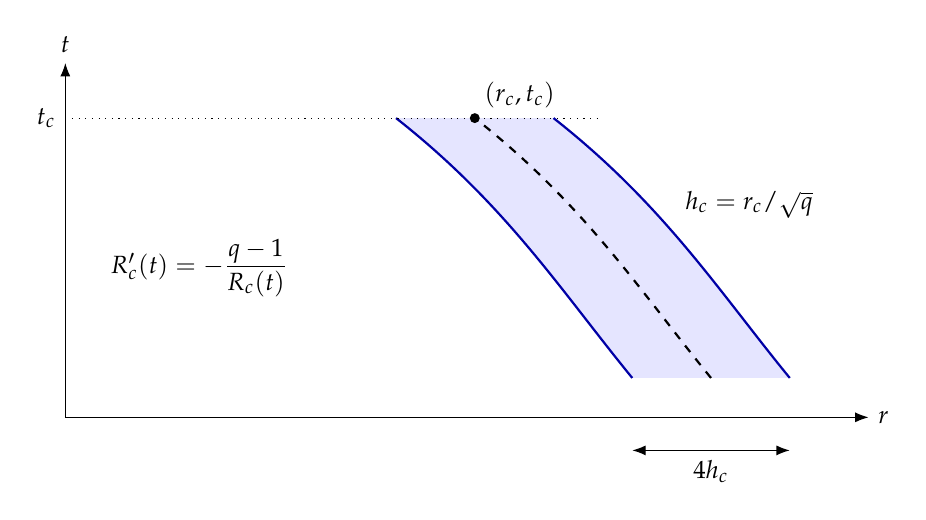
\begin{tikzpicture}[x=1cm,y=1cm,>=Latex,font=\small]
  \draw[->] (0,0)--(10.2,0) node[right] {$r$};
  \draw[->] (0,0)--(0,4.5) node[above] {$t$};
  \fill[blue!10] (7.2,.5) .. controls (6.3,1.6) and (5.6,2.7) .. (4.2,3.8)
      --(6.2,3.8) .. controls (7.6,2.7) and (8.3,1.6) .. (9.2,.5)--cycle;
  \draw[blue!65!black,thick] (7.2,.5) .. controls (6.3,1.6) and (5.6,2.7) .. (4.2,3.8);
  \draw[blue!65!black,thick] (9.2,.5) .. controls (8.3,1.6) and (7.6,2.7) .. (6.2,3.8);
  \draw[dashed,thick] (8.2,.5) .. controls (7.3,1.6) and (6.6,2.7) .. (5.2,3.8);
  \draw[dotted] (0,3.8)--(6.8,3.8);
  \node[left] at (0,3.8) {$t_c$};
  \fill (5.2,3.8) circle (1.8pt);
  \node[above right] at (5.2,3.8) {$(r_c,t_c)$};
  \node[align=left,anchor=west] at (.45,1.9)
    {$R_c'(t)=-\dfrac{q-1}{R_c(t)}$};
  \draw[<->] (7.2,-.42)--(9.2,-.42);
  \node[below] at (8.2,-.42) {$4h_c$};
  \node[anchor=west] at (7.75,2.7) {$h_c=r_c/\sqrt q$};
\end{tikzpicture}

\caption{Schematic image of the fixed cylinder \(P_2\) under
\eqref{eq:moving-cylinder}. Its radial width is \(4h_c\) and its time
length is \(4h_c^2\). Moving with \(R_c'(t)=-(q-1)/R_c(t)\) leaves
a bounded drift after rescaling. The drawing is not to scale.}
\label{fig:drift}
\end{figure}

Since \(R_c'=-(q-1)/R_c\), the function \(H=q(v-1)\), pulled back to
this cylinder, satisfies Lemma~\ref{lem:heat-perturbation} with
\begin{equation}\label{eq:H-coefficients}
\begin{aligned}
a&=z,\\
b&=h_c\left[(q-1)\left(\frac1r-\frac1{R_c}\right)-\frac zr\right],\\
F&=qh_c^2\left[\frac{(q-1)v(1-z)}{r^2}-pv^3u_r^2\right].
\end{aligned}
\end{equation}
Indeed \(|H|\le C_0\), since
\(q|v-1|=q|z-1|/(v+1)\), and \(|a-1|\le C_0/q\).
The apparently large drift is bounded by
\[
\left|h_c(q-1)\left(\frac1r-\frac1{R_c}\right)\right|
=\frac{(q-1)h_c^2|y|}{rR_c}\le C.
\]
For the source use \(qh_c^2=r_c^2\),
\((q-1)|1-z|\le C_0\), and \(r|u_r|\le2\).
All these coefficients and amplitudes are therefore bounded by
one numerical constant. Increasing \(q\) meets its smallness hypothesis.
It follows that \(|H_y|\le C\) on \(P_1\), and hence
\begin{equation}\label{eq:zr-cylinder}
|z_r|=\frac{2v}{qh_c}|H_y|\le\frac{C}{r_c\sqrt q}
\quad\text{on }P_1.
\end{equation}

Differentiate the first equation of~\eqref{eq:sideways}. With \(w=u_r\),
\begin{equation}\label{eq:ur-equation}
w_t=zw_{rr}+\left[z_r+\frac{q-1+z}{r}\right]w_r
+\left[\frac{z_r}{r}-\frac{q-1+z}{r^2}
          +2(p-1)e^{-2u}\right]w.
\end{equation}
On the smaller cylinder \(P_1\), set \(W=r_cw\). Its transformed drift is
\[
b_W=h_c(q-1)(1/r-1/R_c)+h_c(z_r+z/r),
\]
and its zeroth-order coefficient is
\[
c_W=h_c^2\left[z_r/r-(q-1+z)/r^2+2(p-1)e^{-2u}\right].
\]
Equations~\eqref{eq:uniform}, \eqref{eq:cylinder-inclusion}, and
\eqref{eq:zr-cylinder} bound \(|W|\), \(|b_W|\), and \(|c_W|\)
numerically. In particular \(h_c^2(p-1)e^{-2u}\le C\).
Treat \(c_WW\) as a bounded source and apply a fixed rescaled version of
Lemma~\ref{lem:heat-perturbation} on \(P_1\). Evaluating at its center
gives
\[
|W_y(0,0)|=r_ch_c|u_{rr}(r_c,t_c)|\le C.
\]
This proves the second estimate. The first follows from
\eqref{eq:zr-cylinder} at the center. Only the numerical \(C_0\) and
the one-dimensional estimates entered the constants, so neither
\(q\) nor \(k\) occurs in \(C\).
\end{proof}

\subsection{The Ricci norm and its reaction matrix}

The derivative estimates now control the radial sectional curvatures.
The remaining task is algebraic: write the curvature action on invariant
diagonal tensors in coordinates that include their multiplicities in the
norm. This isolates the leading term in \(q\).

The tensor evolution and the evolving metric give
\[
(\dt-\Delta)|\Ric|^2=-2|\nabla\Ric|^2
                         +4\langle\Rm(\Ric),\Ric\rangle.
\]
The inverse-metric derivatives in the squared norm cancel the cubic
Ricci term from the covariant tensor evolution. Kato's inequality then
gives, wherever \(|\Ric|>0\),
\begin{equation}\label{eq:ricci-norm}
(\dt-\Delta)|\Ric|
\le \frac{2}{|\Ric|}\langle\Rm(\Ric),\Ric\rangle.
\end{equation}
For diagonal tensors, our curvature convention is
\(\langle\Rm(D),D\rangle=\sum_{i,j}R_{ijij}D_iD_j\), with
\(R_{ijij}\) the sectional curvature for \(i\ne j\).

\begin{proposition}\label{prop:reaction}
At late times on \(0<r\le\frac18\sqrt\delta\), the reaction quotient
\[
c(x,t)=\frac{2\langle\Rm(\Ric),\Ric\rangle}{|\Ric|^2}
\quad\text{where }|\Ric|>0
\]
satisfies both bounds
\begin{equation}\label{eq:reaction-two}
c\le\frac{2(q-1)+C\sqrt q}{r^2},\qquad
c\le\frac{C_*}{\theta^2}.
\end{equation}
Here \(C\) is independent of \(q,k\); \(C_*\) may depend on the entire
chosen flow. The second bound holds at the pole orbits as well.
Globally at positive \(r\), one also has \(c\le D_1/r^2\) for some
flow-dependent \(D_1>0\).
\end{proposition}

\begin{proof}
The Ricci tensor is diagonal and scalar on each sphere factor. For a tensor
with entries \((\alpha,\beta^{\times p},\chi^{\times q})\), use the
Euclidean coordinates \((\alpha,\sqrt p\beta,\sqrt q\chi)\), so its
norm is the ordinary Euclidean norm. The curvature form has matrix
\begin{equation}\label{eq:reaction-matrix}
\begin{pmatrix}
0&\sqrt p\,h&\sqrt q\,h_q\\
\sqrt p\,h&(p-1)j&\sqrt{pq}\,\mu\\
\sqrt q\,h_q&\sqrt{pq}\,\mu&(q-1)\ell
\end{pmatrix}.
\end{equation}
Indeed its mixed terms are \(2ph\alpha\beta\),
\(2qh_q\alpha\chi\), and \(2pq\mu\beta\chi\); this accounts for
the ordered pairs and all multiplicities.

Using \(r\) as the spatial coordinate,
\begin{equation}\label{eq:curv-sideways}
\begin{gathered}
h=-z(u_{rr}+u_r^2)-\tfrac12z_ru_r,
\qquad h_q=-z_r/(2r),\qquad \mu=-zu_r/r,\\
j=e^{-2u}-zu_r^2,\qquad \ell=(1-z)/r^2.
\end{gathered}
\end{equation}
By Lemmas~\ref{lem:uniform} and~\ref{lem:largeq-derivatives}, after
multiplication by \(r^2\) the diagonal entries of
\eqref{eq:reaction-matrix} are bounded above by
\(0,q-1+C_0,C_0\), respectively. Its off-diagonal entries have sizes
\(O(\sqrt q),O(1),O(\sqrt q)\), respectively, with numerical constants.
The largest eigenvalue is therefore at most \(q-1+C\sqrt q\).
Equation~\eqref{eq:ricci-norm} proves the first bound.
The curvature contraction is bounded in absolute value by a
dimension-dependent constant times \(|\Rm||\Ric|^2\).
Proposition~\ref{prop:full-curvature} gives the other two bounds, including
the bound at a pole by continuity of the geometric curvature tensor.
\end{proof}

\section{Comparison and the scalar-curvature bound}\label{sec:barriers}

We combine the two reaction bounds with small Ricci curvature on
parabolic annuli. The inner comparison gives a spatial Ricci exponent
strictly below one; integrating its square through a scalar supersolution
then gives the required bounded scalar curvature.

For the inner Ricci comparison we will use a positive function of the form
\[
H=\delta^L(r^2+b_0\theta^2)^{-a/2},
\qquad a,L,b_0>0.
\]
Its radial diffusion has leading coefficient \(a(q-1)\), so we require
\(a>2\) to dominate the leading reaction coefficient \(2(q-1)\).
At the cap scale, the identity \(\delta^L=\theta^{L/\sigma}\) makes
its size proportional to \(\theta^{-(a-L/\sigma)}\). We will arrange
that this exponent lies between zero and one, allowing a bounded scalar
barrier to dominate the resulting Ricci-square source. The choices below also make the
parabolic-annulus estimate supply the lateral data for \(H\).

\subsection{Order of the choices}

We now choose one flow to prove Theorem~\ref{thm:main}. Set \(a=5/2\).
Since \(d\to2\) as \(q\to\infty\), choose \(q\) large enough that
\(2<d<a\), all universal thresholds above hold, and
\begin{equation}\label{eq:dimension-margin}
\mathfrak m:=(a-2)(q-1)-C\sqrt q-2a^2-1>0,
\end{equation}
where \(C\) is the universal constant in Proposition~\ref{prop:reaction}.
Next choose a sufficiently large even \(k\) so that, with
\begin{equation}\label{eq:barrier-exponents}
L=k-1,\qquad e=a-L/\sigma=a-d+d/k,
\end{equation}
we have \(0<e<1\), \(\nu>1\), and \(\sigma>1/2\).
These requirements are compatible because \(d>2\).
Define
\[
\xi=\min\{1/8,1/(2\sqrt L)\}.
\]
Choose the tolerances and cutoffs as in Section~\ref{sec:geometry}, and
fix the resulting flow. In particular \(C_*\) and \(D_1\) in
Proposition~\ref{prop:reaction} are now fixed finite numbers.
Only after this step choose \(b_0>0\) so that
\begin{equation}\label{eq:b0-choice}
b_0C_*<\mathfrak m.
\end{equation}
The remaining constants below are chosen for this same flow. Whenever a
later starting time is needed, we restrict to a later slice of the flow
already chosen; we do not repeat the construction or change its parameters.

In Figure~\ref{fig:scales}, \(\Gamma>\xi\) denotes a fixed outer
comparison radius whose size will be chosen in
\eqref{eq:exterior-choices}. The annular estimate is available for
every such fixed radius after moving the starting time later.

\begin{figure}[htbp]
\centering
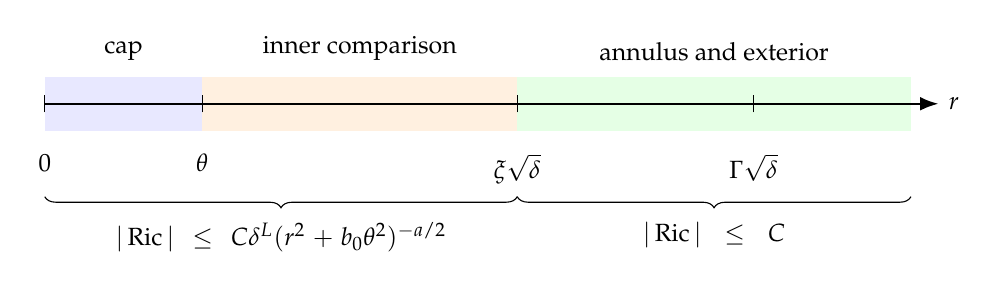
\begin{tikzpicture}[x=1cm,y=1cm,>=Latex,font=\small]
  \fill[blue!9] (0,-.34) rectangle (2,.34);
  \fill[orange!12] (2,-.34) rectangle (6,.34);
  \fill[green!10] (6,-.34) rectangle (11,.34);
  \draw[->,thick] (0,0)--(11.35,0) node[right] {$r$};
  \foreach \x in {0,2,6,9} \draw (\x,-.11)--(\x,.11);
  \node[below=5pt] at (0,-.34) {$0$};
  \node[below=5pt] at (2,-.34) {$\theta$};
  \node[below=5pt] at (6,-.34) {$\xi\sqrt\delta$};
  \node[below=5pt] at (9,-.34) {$\Gamma\sqrt\delta$};
  \node[above] at (1,.42) {cap};
  \node[above,align=center] at (4,.42) {inner comparison};
  \node[above,align=center] at (8.5,.42) {annulus and exterior};
  \draw[decorate,decoration={brace,amplitude=4pt,mirror}] (0,-1.18)--(6,-1.18);
  \node[below,align=center,text width=6.2cm] at (3,-1.38)
     {$|\Ric|\le C\delta^L(r^2+b_0\theta^2)^{-a/2}$};
  \draw[decorate,decoration={brace,amplitude=4pt,mirror}] (6,-1.18)--(11,-1.18);
  \node[below,align=center,text width=4.7cm] at (8.5,-1.38)
     {$|\Ric|\le C$};
\end{tikzpicture}

\caption{The comparison regions at a late time, shown on a schematic
radius axis. The cap scale \(\theta\) is much smaller than the
parabolic scale \(\sqrt\delta\). The inner Ricci estimate bridges these
scales. Fixed parabolic-annulus control supplies lateral data for both
the inner and exterior comparisons; \(\Gamma\) is chosen later in
\eqref{eq:exterior-choices}.}
\label{fig:scales}
\end{figure}

\subsection{The inner Ricci estimate}

\begin{proposition}\label{prop:ricci-barrier}
There is a constant \(C\) such that, at all sufficiently late times,
\begin{equation}\label{eq:inner-ricci}
|\Ric|\le C\delta^L(r^2+b_0\theta^2)^{-a/2}
\qquad(0\le r\le\xi\sqrt\delta).
\end{equation}
In particular,
\begin{equation}\label{eq:ricci-power}
|\Ric|\le Cr^{-e}\qquad(0<r\le\xi\sqrt\delta).
\end{equation}
\end{proposition}

\begin{proof}
Put \(D_0=r^2+b_0\theta^2\) and \(H=\delta^LD_0^{-a/2}\).
This is a positive smooth geometric function on both closed caps,
including their pole orbits, because \(r^2\) is smooth there.
Using \(\theta_t=-\sigma\theta/\delta\) and
Equation~\eqref{eq:operator}, direct differentiation gives
\begin{equation}\label{eq:inner-barrier-computation}
\begin{split}
\frac{\D H}{H}
&=-\frac L\delta+\frac{a\sigma b_0\theta^2}{\delta D_0}
 +\frac{a(q-1)+2az}{D_0}-\frac{a(a+2)zr^2}{D_0^2}\\
&\ge-\frac L\delta+\frac{a(q-1)-a^2z}{D_0}.
\end{split}
\end{equation}
The first line has a nonnegative extra time term, and \(r^2\le D_0\)
gives the second. The identities extend to a pole by continuity; in
particular the apparent \(r^{-1}H_r\) term has a finite limit.

In the indicated region \(z\le2\) for large \(q\), and
\[
LD_0/\delta\le L\xi^2+Lb_0\delta^{2\sigma-1}\le1
\]
at sufficiently late times. Where \(|\Ric|>0\) and \(r>0\), the two
bounds in~\eqref{eq:reaction-two} imply
\[
cD_0=cr^2+b_0c\theta^2
\le2(q-1)+C\sqrt q+b_0C_*.
\]
Both inequalities may be added even if \(c\) is negative. At a pole,
the second reaction bound alone implies the same upper bound for
\(cD_0\). Therefore
\begin{equation}\label{eq:strict-ricci-super}
\frac{\D H}{H}-c
\ge\frac{-1+a(q-1)-2a^2-2(q-1)-C\sqrt q-b_0C_*}{D_0}>0
\end{equation}
by~\eqref{eq:dimension-margin} and~\eqref{eq:b0-choice}.

On the moving lateral boundary \(r=\xi\sqrt\delta\),
\[
H=\delta^{L-a/2}
    (\xi^2+b_0\delta^{2\sigma-1})^{-a/2}
\asymp\delta^{L-a/2}.
\]
Lemma~\ref{lem:annuli} and \(\nu=k-d/2\) give
\begin{equation}\label{eq:lateral-ratio}
\frac{|\Ric|}{H}\le C\delta^{\nu-1-(L-a/2)}
=C\delta^{(a-d)/2}.
\end{equation}
This ratio is uniformly bounded at late times. Choose a sufficiently
late fixed starting time \(t_0\). On that compact starting slice, \(H\)
has a positive minimum on the caps, so a single multiple of \(H\)
strictly dominates both initial and lateral data for every subsequent
compact time slab.

At a first contact of \(|\Ric|\) with this positive barrier, the Ricci
norm is nonzero and hence smooth nearby. Equation~\eqref{eq:ricci-norm}
and the strict inequality~\eqref{eq:strict-ricci-super} rule out the
contact by the maximum principle. This argument also applies at a pole,
which is interior to the smooth manifold. It proves~\eqref{eq:inner-ricci}
with one multiplier for all times \(t_0\le t<T\).

Finally \(\delta^L=\theta^{L/\sigma}=\theta^{a-e}\), with \(a-e>0\).
For \(r\ge\theta\),
\[
H\le\theta^{a-e}r^{-a}\le r^{-e}.
\]
For \(0<r\le\theta\),
\[
H\le b_0^{-a/2}\theta^{-e}\le b_0^{-a/2}r^{-e}.
\]
These prove~\eqref{eq:ricci-power}.
\end{proof}

\subsection{A scalar barrier at the pole}

\begin{proposition}\label{prop:scalar-inner}
The scalar curvature is uniformly bounded above on
\(0\le r\le\xi\sqrt\delta\) at late times.
\end{proposition}

\begin{proof}
For a real exponent \(\alpha\), Equation~\eqref{eq:operator} gives
\begin{equation}\label{eq:power-operator}
\D(r^\alpha)=-\alpha(q-1+\alpha z)r^{\alpha-2}
\qquad(r>0).
\end{equation}
Put \(\ell_0=2-2e\in(0,2)\). In particular,
\begin{equation}\label{eq:scalar-powers}
\D(-r^{\ell_0})=\ell_0(q-1+\ell_0z)r^{-2e},
\qquad \D(r^{-1})=(q-1-z)r^{-3}.
\end{equation}
Write \(|\Ric|\le K_Rr^{-e}\) as in Proposition~\ref{prop:ricci-barrier}.
Choose
\[
C_2\ge\frac{2K_R^2}{\ell_0(q-1)}.
\]
Since \(0\le z\le2<q-1\), every function
\begin{equation}\label{eq:scalar-barrier}
S_\varepsilon=C_1-C_2r^{\ell_0}+\varepsilon r^{-1},
\qquad \varepsilon>0,
\end{equation}
satisfies \(\D S_\varepsilon\ge2|\Ric|^2\) at positive radii in the
inner region.

Choose one late starting time \(t_0\) and let
\(\rho_0=\xi\sqrt{T-t_0}\). Smoothness bounds scalar curvature on
the starting slice by a constant \(K_0\). On the moving lateral boundary,
Lemma~\ref{lem:annuli}, \(\nu>1\), and
\(|R|\le\sqrt{m+1}|\Ric|\) give a uniform upper bound \(K_\partial\).
The choice
\begin{equation}\label{eq:C1-choice}
C_1>\max\{K_0,K_\partial\}+C_2\rho_0^{\ell_0}
\end{equation}
therefore dominates the initial and lateral scalar data for every
\(\varepsilon>0\).

Fix \(\varepsilon>0\) and \(t_1<T\). Scalar curvature is bounded on
the compact slab \([t_0,t_1]\). For sufficiently small \(\eta>0\), the
level \(r=\eta\) lies in the regular inner region throughout that slab
and \(\varepsilon/\eta\) makes \(S_\varepsilon\) dominate its scalar
data. Apply comparison to \(R-S_\varepsilon\) on
\[
\{(x,t):t_0\le t\le t_1,\ \eta\le r(x,t)\le\xi\sqrt{T-t}\}.
\]
The moving outer boundary is regular in the monotone inner region.
Both initial and lateral boundaries have been controlled, so the usual
interior first-maximum argument applies. Let \(\eta\downarrow0\).
This proves \(R\le S_\varepsilon\) at every positive radius on the slab.

Only the auxiliary excision radius depends on \(\varepsilon,t_1\);
the constants in~\eqref{eq:C1-choice} do not. Letting the slab range up to
\(T\) and then sending \(\varepsilon\downarrow0\) pointwise gives
\[
R\le C_1-C_2r^{\ell_0}\le C_1\qquad(r>0).
\]
At every fixed time \(t<T\), continuity gives the same bound at the
pole orbits. No smoothness of \(r^{\ell_0}\) at the pole or uniform
regularity at \(t=T\) was used.
\end{proof}

\subsection{The exterior and the maximal time}

\begin{proposition}\label{prop:exterior}
There is a constant \(C\) such that
\(|\Ric|\le C\) on \(r\ge\xi\sqrt\delta\) at late times.
\end{proposition}

\begin{proof}
Choose \(b_1>2D_1+1\), where \(D_1\) is the global reaction constant
in Proposition~\ref{prop:reaction}, and choose
\begin{equation}\label{eq:exterior-choices}
\Gamma>\xi,\qquad \Gamma^2\ge\max\{2b_1,4(q-1)\}.
\end{equation}
On the entire geometric exterior \(r\ge\Gamma\sqrt\delta\), put
\(H_o=1-b_1\delta/r^2\). This is smooth across the equator and satisfies
\(1/2\le H_o\le1\). Equation~\eqref{eq:operator} gives
\begin{equation}\label{eq:outer-barrier}
\D H_o=\frac{b_1}{r^2}
\left[1-\bigl(2(q-1)-4z\bigr)\frac{\delta}{r^2}\right]
\ge\frac{b_1}{2r^2}>\frac{D_1H_o}{r^2}.
\end{equation}
Here only \(z\ge0\) was needed; no global smallness of \(z-1\) is
required.

The fixed parabolic radius \(\Gamma\) eventually lies in the region of
Lemma~\ref{lem:annuli}. The annular estimate and \(\nu>1\) bound \(|\Ric|\) on
the moving lateral boundary uniformly. On a sufficiently late starting
slice, compactness and \(H_o\ge1/2\) allow one multiplier to dominate
the initial data. The same first-contact argument as in
Proposition~\ref{prop:ricci-barrier} proves \(|\Ric|\le CH_o\le C\)
throughout the exterior. The equator is interior, since both hemispheres
are included. On the remaining fixed annulus
\(\xi\le r/\sqrt\delta\le\Gamma\), use Lemma~\ref{lem:annuli}
directly.
\end{proof}

\begin{proof}[Proof of Theorem~\ref{thm:main}]
Take the single flow selected at the start of Section~\ref{sec:barriers}.
Propositions~\ref{prop:scalar-inner} and~\ref{prop:exterior} give a
uniform scalar upper bound on all of \(M\) for sufficiently late times.
There are only finitely many required starting-time restrictions, and
every parameter and constant has already been fixed, so a common such
time exists. Earlier times form a compact smooth interval and contribute
a finite bound. Lemma~\ref{lem:gradients} supplies the scalar lower bound.
Thus \(\sup_{M\times[0,T)}|R|<\infty\).

By Lemma~\ref{lem:pole-size}, \(\phi(0,t)\le C\theta(t)\to0\).
At a pole orbit, smoothness gives \(\phi_s=0\). Since \(p=2\), a
two-plane tangent to the \(\Sp^p\) orbit has sectional curvature
\[
j(0,t)=\phi(0,t)^{-2}\longrightarrow\infty.
\]
Consequently \(\max_M|\Rm|\to\infty\). A smooth extension on the same
compact manifold would bound curvature on a compact time neighborhood
of \(T\), which is impossible. The constructed flow exists smoothly for
every \(t<T\); closed-manifold uniqueness therefore identifies \(T\)
with the maximal existence time for its smooth initial metric. The product
\(\Sp^2\times\Sp^{q+1}\) is closed, connected, and has dimension
\(q+3\ge4\), as required.
\end{proof}

\begin{corollary}[Curvature rates in a fixed dimension]\label{cor:rates}
For every sufficiently large integer \(q\), set
\[
d_q=\frac{q+1-\sqrt{(q+1)(q-7)}}2.
\]
For every sufficiently large even integer \(k\), with the threshold
allowed to depend on \(q\), there is a smooth Ricci flow on
\(\Sp^2\times\Sp^{q+1}\) with finite maximal time \(T\), uniformly
bounded scalar curvature, and constants \(0<c\le C<\infty\) such that
\[
c(T-t)^{-2k/d_q}\le\max_M|\Rm|(\cdot,t)
\le C(T-t)^{-2k/d_q}
\]
for all sufficiently late times. In particular, one fixed dimension
admits such flows with an unbounded discrete set of power-law Type-II
curvature exponents. The flow, \(T\), and the constants may depend on
\(q\) and \(k\).
\end{corollary}

\begin{proof}
Every threshold used to choose \(q\) at the beginning of this section
is independent of \(k\). Once such a \(q\) is fixed, all sufficiently
large even \(k\) satisfy the requirements in
\eqref{eq:barrier-exponents}; Proposition~\ref{prop:input} then permits
the remaining choices. The preceding comparisons apply to each resulting
flow, with constants that may depend on it.

Here \(d=d_q\) and \(\theta=(T-t)^{k/d_q}\).
Proposition~\ref{prop:full-curvature} gives
\(\max_M|\Rm|\le C\theta^{-2}\).
At either pole orbit, Lemma~\ref{lem:pole-size} gives
\(\phi(0,t)\le C\theta\), and the tangential sectional curvature is
\(j(0,t)=\phi(0,t)^{-2}\). Hence
\(\max_M|\Rm|\ge c\theta^{-2}\).
These are the claimed two-sided bounds. Since \(2k/d_q>1\) and tends
to infinity with \(k\), the flows are Type~II and their exponents are
unbounded with \(q\) fixed.
\end{proof}

\begin{thebibliography}{99}
\raggedright

\bibitem{AIK2015}
S.~Angenent, J.~Isenberg, and D.~Knopf,
\emph{Degenerate neckpinches in Ricci flow},
J. Reine Angew. Math. \textbf{709} (2015), 81--117.
\href{https://arxiv.org/abs/1208.4312v1}{arXiv:1208.4312v1}.

\bibitem{AK2004}
S.~Angenent and D.~Knopf,
\emph{An example of neckpinching for Ricci flow on \(S^{n+1}\)},
Math. Res. Lett. \textbf{11} (2004), no.~4, 493--518.
\href{https://web.ma.utexas.edu/users/danknopf/Neckpinch.pdf}{Author's text};
\href{https://web.ma.utexas.edu/users/danknopf/Corrigendum.pdf}{corrigendum}.

\bibitem{Bamler2018}
R.~H. Bamler,
\emph{Convergence of Ricci flows with bounded scalar curvature},
Ann. of Math. (2) \textbf{188} (2018), no.~3, 753--831.
\href{https://doi.org/10.4007/annals.2018.188.3.2}{doi:10.4007/annals.2018.188.3.2}.

\bibitem{Bohm1999}
C.~B\"ohm,
\emph{Non-compact cohomogeneity one Einstein manifolds},
Bull. Soc. Math. France \textbf{127} (1999), no.~1, 135--177.
\href{https://doi.org/10.24033/bsmf.2345}{doi:10.24033/bsmf.2345}.

\bibitem{CaoZhu2006}
H.-D. Cao and X.-P. Zhu,
\emph{A complete proof of the Poincar\'e and geometrization conjectures---application
of the Hamilton--Perelman theory of the Ricci flow},
Asian J. Math. \textbf{10} (2006), no.~2, 165--492.
\href{https://www.renyi.hu/~stipsicz/perelman/cao-zhu.pdf}{Full text}.

\bibitem{GuZhu2008}
H.-L.~Gu and X.-P. Zhu,
\emph{The existence of Type II singularities for the Ricci flow on
\(S^{n+1}\)},
Comm. Anal. Geom. \textbf{16} (2008), no.~3, 467--494.
\href{https://arxiv.org/abs/0707.0033v1}{arXiv:0707.0033v1}.

\bibitem{Hamilton1995}
R.~S. Hamilton,
\emph{The formation of singularities in the Ricci flow},
Surveys in Differential Geometry, Vol.~II (Cambridge, MA, 1993),
International Press, Cambridge, MA, 1995, 7--136.
\href{https://intlpress.com/site/pub/files/_fulltext/journals/sdg/1993/0002/0001/SDG-1993-0002-0001-a002.pdf}{Full text}.

\bibitem{Krylov2006}
N.~V. Krylov,
\emph{Parabolic equations with VMO coefficients in spaces with mixed norms},
\href{https://arxiv.org/abs/math/0610955v1}{arXiv:math/0610955v1}, 2006.
Theorem numbering refers to this version.
Published as \emph{Parabolic equations with VMO coefficients in Sobolev
spaces with mixed norms}, J. Funct. Anal. \textbf{250} (2007), no.~2,
521--558.
\href{https://doi.org/10.1016/j.jfa.2007.04.003}{doi:10.1016/j.jfa.2007.04.003}.

\bibitem{LSU1968}
O.~A. Ladyzhenskaya, V.~A. Solonnikov, and N.~N. Ural'tseva,
\emph{Linear and Quasi-linear Equations of Parabolic Type},
Translations of Mathematical Monographs, vol.~23,
American Mathematical Society, Providence, RI, 1968;
corrected reprint, 1988.
\href{https://doi.org/10.1090/mmono/023}{doi:10.1090/mmono/023}.

\bibitem{Sesum2005}
N.~\v{S}e\v{s}um,
\emph{Curvature tensor under the Ricci flow},
Amer. J. Math. \textbf{127} (2005), no.~6, 1315--1324.
\href{https://doi.org/10.1353/ajm.2005.0042}{doi:10.1353/ajm.2005.0042}.

\bibitem{Shi1989}
W.-X. Shi,
\emph{Deforming the metric on complete Riemannian manifolds},
J. Differential Geom. \textbf{30} (1989), no.~1, 223--301.
\href{https://doi.org/10.4310/jdg/1214443292}{doi:10.4310/jdg/1214443292}.

\bibitem{Stolarski2019}
M.~Stolarski,
\emph{Curvature Blow-up in Doubly-warped Product Metrics Evolving by Ricci Flow},
\href{https://arxiv.org/abs/1905.00087v1}{arXiv:1905.00087v1}, 2019.
All numbered source references in this paper use this version.
Published in Mem. Amer. Math. Soc. \textbf{295} (2024), no.~1470.
\href{https://doi.org/10.1090/memo/1470}{doi:10.1090/memo/1470}.

\bibitem{Wang2012}
B.~Wang,
\emph{On the conditions to extend Ricci flow (II)},
Int. Math. Res. Not. IMRN \textbf{2012}, no.~14, 3192--3223.
\href{https://doi.org/10.1093/imrn/rnr141}{doi:10.1093/imrn/rnr141}.
\href{https://arxiv.org/abs/1107.5107v1}{arXiv:1107.5107v1};
theorem numbering refers to this preprint version.

\end{thebibliography}

\end{document}
